
\documentclass[runningheads]{llncs}

\usepackage{amssymb}
\usepackage[english]{babel}
\usepackage[utf8]{inputenc}
\setcounter{tocdepth}{3}
\usepackage{graphicx}

\usepackage{url}
\urldef{\mailsa}\path|{jrra,ksma,atka}@itu.dk|
\newcommand{\keywords}[1]{\par\addvspace\baselineskip
\noindent\keywordname\enspace\ignorespaces#1}
\graphicspath{{images/}}

\begin{document}

\mainmatter  % start of an individual contribution

% first the title is needed
\title{Model-Driven Development Project:\\ Modelling, Domain-Specific Language\\ and Code Generation}

% a short form should be given in case it is too long for the running head
\titlerunning{Model-Driven Development Project}

\author{Kristian Støving Mørk Andersen \and \\ Athanasios Kastanidis \and \\ Jacob Romme Rasmussen}
%
\authorrunning{Model-Driven Development Project}

\institute{\mailsa\\}

\toctitle{Lecture Notes in Computer Science}
\tocauthor{Authors' Instructions}
\maketitle


\begin{abstract}
This paper covers the process of modelling and structuring a domain-specific language (DSL). By being smaller and easier to understand than a general-purpose programming language, a DSL makes it possible for a larger amount of people to write programs in the domain. This paper focuses on the survey domain. Having performed a domain analysis, we present a survey-specific language including its own editor and compiler. Code is automatically generated from the surveys written in the DSL and targets multiple platforms, namely the Android mobile platform and a Web platform. 
\end{abstract}

\section{Introduction}
This paper describes the design and implementation of a Domain Specific Language for generating survey applications. The purpose of the project is to design a language that can be used by a person with no prior programming experience to define surveys. Within the domain, a DSL is substantially easier to use and understand compared to general-purpose programming languages \cite{mernik}. By exposing the DSL to people who understand the domain, you allow for better communication between the programmer, who writes the code for the DSL, and the customer, that is - the domain expert \cite{fowler}. 

The surveys defined in the DSL can then be used to generate applications for answering surveys on multiple platforms. This reduces the amount of code duplication a programmer would generally encounter while writing a survey application for multiple platforms. In turn this also reduces the time development takes. Most importantly the survey DSL along with the code generation tool can be used to generate and endless number of survey applications without rewriting any code. 

The first step towards designing a DSL is to perform a domain analysis. The analysis provides the neccessary information to model and design the language. Code can be generated from a program written in the DSL by using the dynamic survey-specific information contained in the program and inserting it into several static templates. After writing a valid survey, the generated code is immediately accesible to the user. 

\section{System Overview}
The flow of the system is visualized in fig. \ref{fig:flow} showing where and when various programming-specific tasks take place.
\begin{figure}
\centering
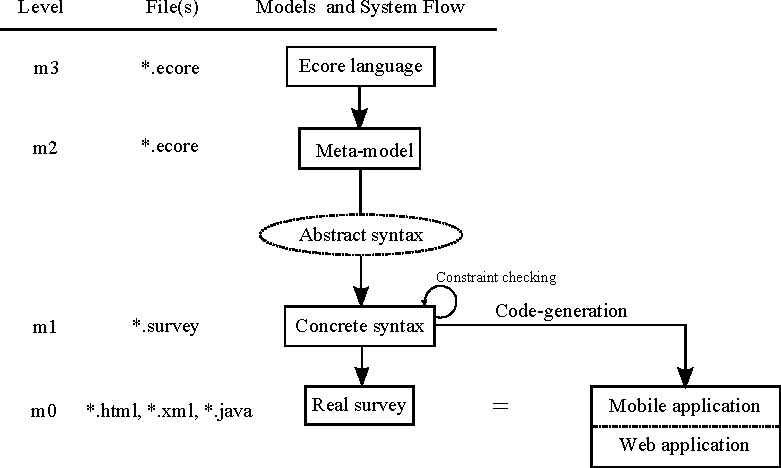
\includegraphics[height=6cm]{systemflow}
\caption{A figure depicting the flow of the system.}
\label{fig:flow}
\end{figure}
The meta-model of our language written in the Ecore language is where the structure and relations of the system are defined. Together with the abstract syntax, the structure and relations of the meta-model are passed to the concrete syntax. At this point, a language-specific file (*.survey) is the center of attention. Constraints are checked against this file and code is generated from this file if the constraints are satisfied. The actual survey is the endpoint of the system flow and can take on different forms. In our case, a real survey consists of files that provide the core of an Android application and a Web application. 

From a target user's viewpoint, he writes his survey in the editor built in Eclipse following the survey program syntax. If no constraints are violated, code is generated from his survey when he saves the program. If he wants to put the generated Android application code to use, he has to create a new Android project and add the generated file. The application should be ready for deployment on an Android phone. In the case of a Web application he has to move the generate file to his webserver and they should be ready for use.

\section{Language Requirements and Design}
\label{sec:requirements_and_design}
%Domain analysis and the meta-model
%Concrete-syntax (interesting aspects of the grammar)
%How and what design principles you followed? (cite literature) \\
When performing the domain analysis we searched for the most popular online survey sites and chose to use the survey templates provided by Surveymonkey \cite{surveymonkey} and Obsurvey \cite{obsurvey} as inspiration. Due to their popularity, the language is specifically designed to support their survey design. Their surveys span a variety of different types of questions. Multiple answers can be given to some questions, while others only allow a single answer. Most answers are preset, while some allows the user to insert free text. A question can contain answers of both types. The questions are either listed on a single page or divided into several pages. A question can depend on previous answers meaning it is only shown if a certain answer was chosen earlier. This is useful when some answers make the following questions irrelevant. The combined functionality of the investigated surveys lead to the following requirements for the survey system:
\begin{itemize}
\item A survey must contain at least one question. 
\item A question has a type indicating the amount and types of answers allowed. 
\item A question can require specific previous answers and should only be made available if all the required answers were chosen by the user. 
\item Multiple choice questions allow users to choose multiple predefined answers.
\item Single choice questions should only allow a single answer. 
\item Open questions do not contain any predefined answers but allow a user to define the answer themselves. 
\item An open question must contain a single open(not predefined) answer.
\end{itemize}
When defining the elements of the language, we chose to follow a set of guidelines by Karsai et al. \cite{karsai}. The main guidelines being
\begin{quotation}
\emph{Reflect only the necessary domain concepts.} [...] \emph{Keep it simple.} [...] \emph{Avoid unnecessary generality.} [...] \emph{Limit the number of language elements.}
\end{quotation}
\begin{figure}[h]
\centering
 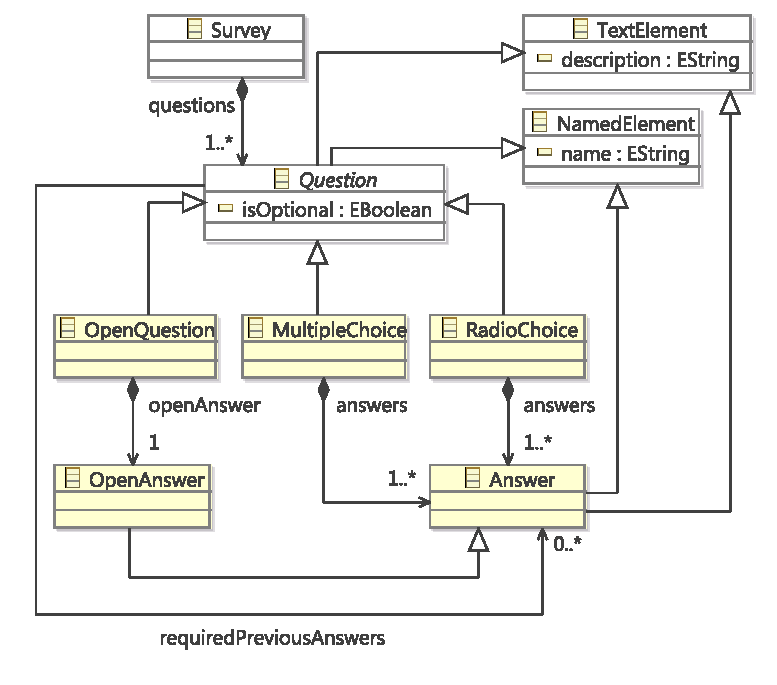
\includegraphics[height=6.2cm]{metamodel}
\caption{A figure depicting the metamodel of the DSL.}
\label{fig:mmod}
\end{figure}
During the language design phase, simplicity is one of the main goals \cite{karsai}. Along with the design guidelines, this is hopefully reflected in the model which contains a minimum number of entities while still capturing the essence of the survey domain.  
The structure of the meta-model shown in fig. \ref{fig:mmod}. The \textsf{Survey} root element contains one or more questions. The \textsf{Question} entity is split into three subentities denoting the type of question. An alternative approach would be to merge the \textsf{MultipleChoice} and \textsf{RadioChoice} entities and use an enumeration to describe a question type attribute. However, we argue that it is visually more pleasing to have the distinct separation displayed in the model. A \textsf{Question} contains one or more references to answers denoting the relevancy of the question. A constraint is run on the model, checking that no question requires one of its own answers. The model provides the basis for the abstract syntax of the domain-specific language, which is used to write a survey in concrete syntax. 

We will explain our concrete syntax based on the example program shown in fig. \ref{fig:concrete}.
\begin{figure}
\centering
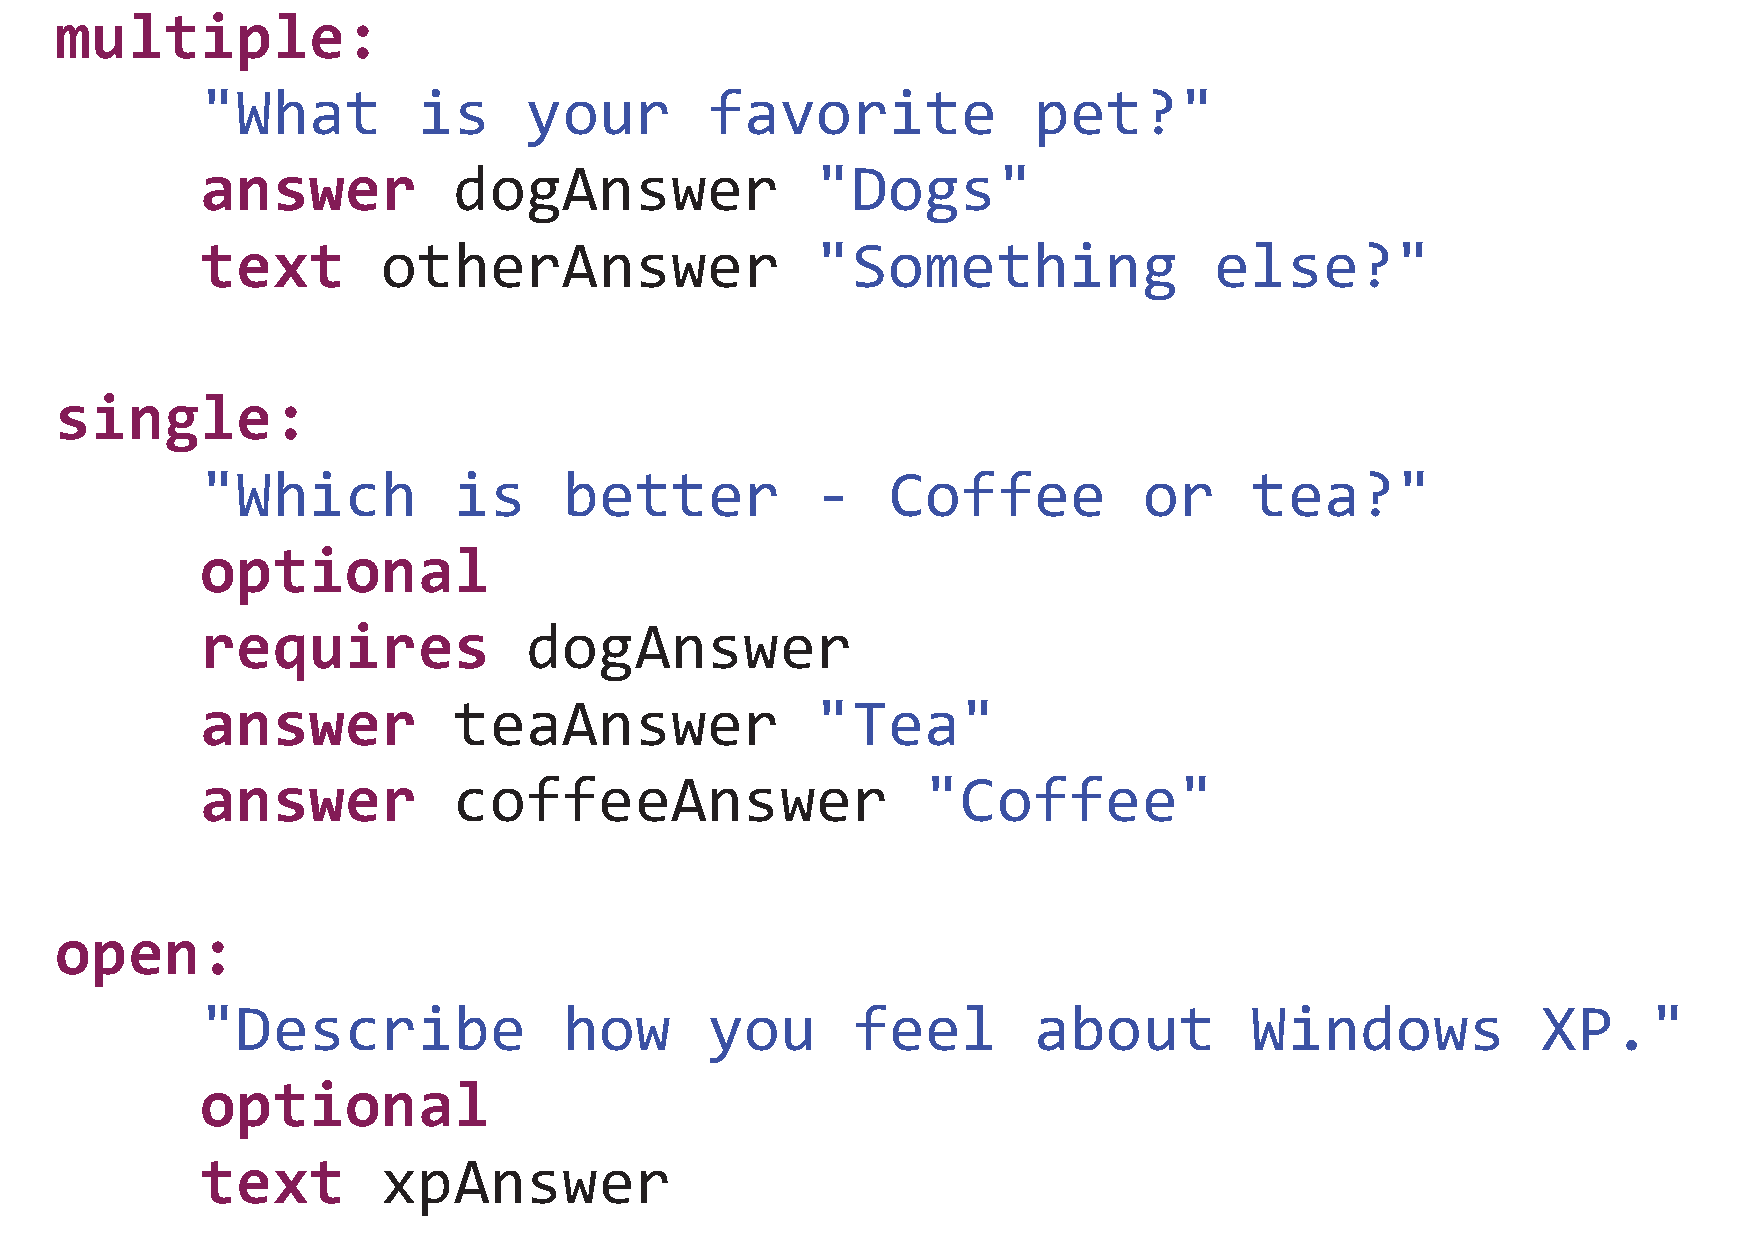
\includegraphics[height=5cm]{concrete}
\caption{Concrete syntax example.}
\label{fig:concrete}
\end{figure}

\noindent
It is in such a file that the target user writes their surveys. The file contains one or more question-segments. A segment defines the type of the question followed by a surveyor-defined description - the actual question to be read by the surveyee. The \textsf{optional}-keyword is used to indicate if the question in the given segment is optional. If the question segment requires specific previous answer the \textsf{requires}-keyword is used followed by the identifier of the answer required. The remainder of the segment contains a list of answers starting with the \textsf{answer}-keyword, followed by an identifier and a description (the actual predefined answer). The identifier is only used internally when referencing the answer from somewhere else in the program. The referencing of answers is used when \emph{requiring} that certain answers have been chosen by the surveyee in order for the question to be relevant. The naming of the keywords are chosen specifically to capture the essence of their functionality and be easily understandable by anyone with no prior programming experience. When designing the concrete syntax of a domain-specific language, Karsai et al. \cite{karsai} recommends that one should
\begin{quotation}
 \emph{Adopt existing notations domain experts use.} [...] \emph{Use descriptive notations.}
\end{quotation}
Thus, many of the keywords are names of concepts used in the survey domain. The colon is commonly known to explain or define the preceeding element - here it is used to indicate the start of the definition and contents of a question. The overall goal of the concrete syntax design is that only minor knowledge about surveys is enough to be able to use the DSL with ease. 

\section{Language Implementation and Code Generation}
We have chosen to model our language as an external DSL such that it can be independent of any other language. The survey DSL itself is implemented using Xtext \cite{xtext}, an Open Source framework for development of programming languages and DSL's. Xtext is highly integrated with the Eclipse IDE. When developing a language using Xtext it is possible to generate Eclipse plugins which offer a fully integrated IDE within Eclipse, allowing the user to benefit from syntax highlighting, error messaging and other features. By using Xtext for our DSL we gain these capabilities with only little effort. Using the template capabilities of Xtend \cite{xtend}, we can generate code from instances created in our language.

\subsection{Android implementation}
The first part of the code generation generates an Android application for answering a survey. Because Android runs Java it would be easy to choose to run the DSL as interpreted language in the Android application. This could on the other hand make the app slower on the computationally constrained hardware Android runs within. It would also be harder to read the files of the interpreted language if the format or language changes since those changes would also need to be incorporated on the Android platform side. Instead we have chosen to generate native Java code for the Android app to make it fast and easily adaptable to other platforms. The flow of the Android application code generation is shown in fig. \ref{fig:appgen}. The generator receives a survey and generates an activity file. The user has to manually insert the generated file into an Android Project. Ideally, we would have preferred to generate the entire Android project required for an Android Application making the process denoted by the dashed arrows automatic. 
\begin{figure}
\centering
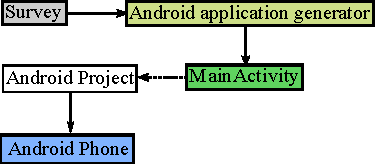
\includegraphics[height=2.5cm]{appgen}
\caption{A figure displaying the code generation flow of the Android application implementation.}
\label{fig:appgen}
\end{figure}
The survey is displayed with one question on each page. That way it is easier to show the next question based on the answer of the the current answer. Once all the questions have been filled out the activity composes an email with all the answers that can be send to the survey creator.

\begin{figure}[h]
\centering
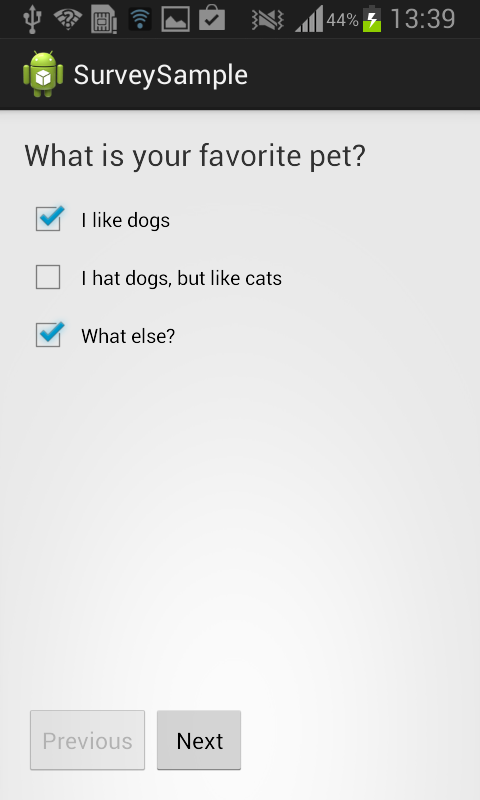
\includegraphics[width=4cm]{android_screenshot}
\caption{A screenshot of the android application.}
\label{fig:android_screenshot}
\end{figure}

The Android application has three classes that represent \texttsf{Survey}, \textsf{Question}, \textsf{Answer} from the meta model. It also has a few view fragments and a single activity that controls the flow of the application. The code generator only needs to generate a single method for the \textsf{MainActivity} that instantiates the classes from the domain model. This way, the amount of dynamic code in the Android application stays minimal.

In fig. \ref{fig:android_screenshot} a screenshot of the working Android application is shown. The application is generated from the survey language example shown in figure \ref{fig:concrete}.

\subsection {HTML Implementation}
The second part of the code generation generates a Web application for answering a survey. Web interfaces are ideal when wanting to span a variety of platforms and systems, providing a uniform presentation layer while leaving the platform- and Operating System-specific implementation to the browser. While a Web application can be less interactive and intuitive to the end-user, the ease of deployment (the web page does not require installation like the android application) means that users that might be discouraged from going through an installation process could be convinced to click on a link in their browsers and complete an online survey. At the same time a web page provides new challenges, since separating unique users and offering any sort of intermediate persistency ("pausing" a survey and returning to it at a later time) increase the complexity requirements on the sever-side. 
\begin{figure}
\centering
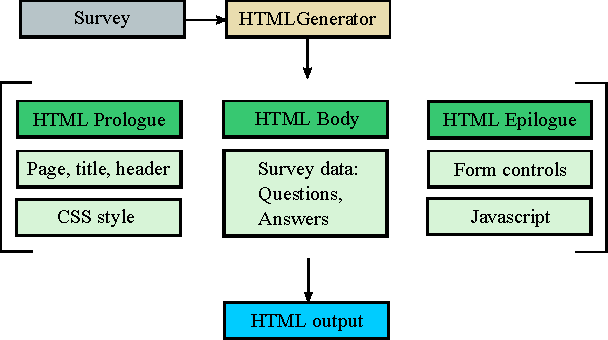
\includegraphics[height=4cm]{htmlgen}
\caption{A figure displaying the code generation flow of the HTML implementation.}
\label{fig:htmlgen}
\end{figure}
The flow of the HTML implementation is depicted in fig. \ref{fig:htmlgen}. The HTML code generation works as a single pipeline, each phase of the code, Prologue, Body and Epilogue are added together to produce the final result. Semantics and presentation is mixed through the code.  

In the HTML Prologue we can find the basic header of an HTML file, defining things like the page title, meta tags to assist search engines in finding the page. The page's style is also defined in the header using CSS, which minimizes to a certain extend how much the actual content is mixed with presentation logic. The vast majority of the Prologue is static until we reach the javascript logic which controls the final submission of the form. In this script all preconditions are checked (all non-optional questions have at least an answer) which allows the e-mail with the answers to be sent. 

The main part of the HTML is the Body, which holds all the actual text with the questions and possible answers. This is the part where controlling logic, presentation layer and user content are combined together. Depending on the type of the question a different type of layout is rendered to the page, with different type of HTML input controls. The HTML tags are configured with the correct IDs for each answer, and the type of input elements that will be rendered to the page will "force" correctness (e.g. only a single Radio button can be selected in a group, so only a single answer can be given). Much like the page itself, each question in itself is a small pipeline with its own Prologue, Body and Epilogue. The Prologue consists of the question description and whether it is optional or not. The Body consists of the different answers and the Epilogue just ensures that all HTML tags are appropriately "closed".  

Finally the HTML  Epilogue will provide the final controls of the form which allow the user to either submit his answers or reset the page, together with the appropriate hooks to run the JavaScript code before the form is passed to the user's e-mail client.

\section{Testing}
The meta-model has been tested manually by creating dynamic instances of the model. We attempted to create both valid and invalid instances to check if the model can satisfy the requirements. This procedure helped us catching errors earlier in the process.

Initially the concrete syntax was only tested by manually writing survey instances in the Eclipse editor. This was done to check that the model structure was correctly preserved and interpreted by the compiler. A few more testing procedures have been added to contribute to the functionality of the system.
\subsubsection{Constraints}
Constraints are checked automatically on a concrete instance of our language before any code is generated. The constraints are included in the validation-package of the DSL project and checked in the generation package of the DSL project. The constraints guard against
\begin{itemize}
\item \emph{circularity}: no question contains one of their own answers in the list of required previous answers.
\item \emph{empty strings}: no question or answer has an empty description.
\end{itemize}
Code is only generated when all constraints are satisfied. If that is not the case, a message is printed to the console informing the user about the constraint violation(s). Saving the program in fig. \ref{fig:concretefail} does not generate any code and will print the following message in the console window:

\noindent
\texttt{Constraints violated. Either a question contains a reference to its own answer or a description string is empty.}

This is because the second question is circular by requiring an answer contained in itself.
\begin{figure}
\centering
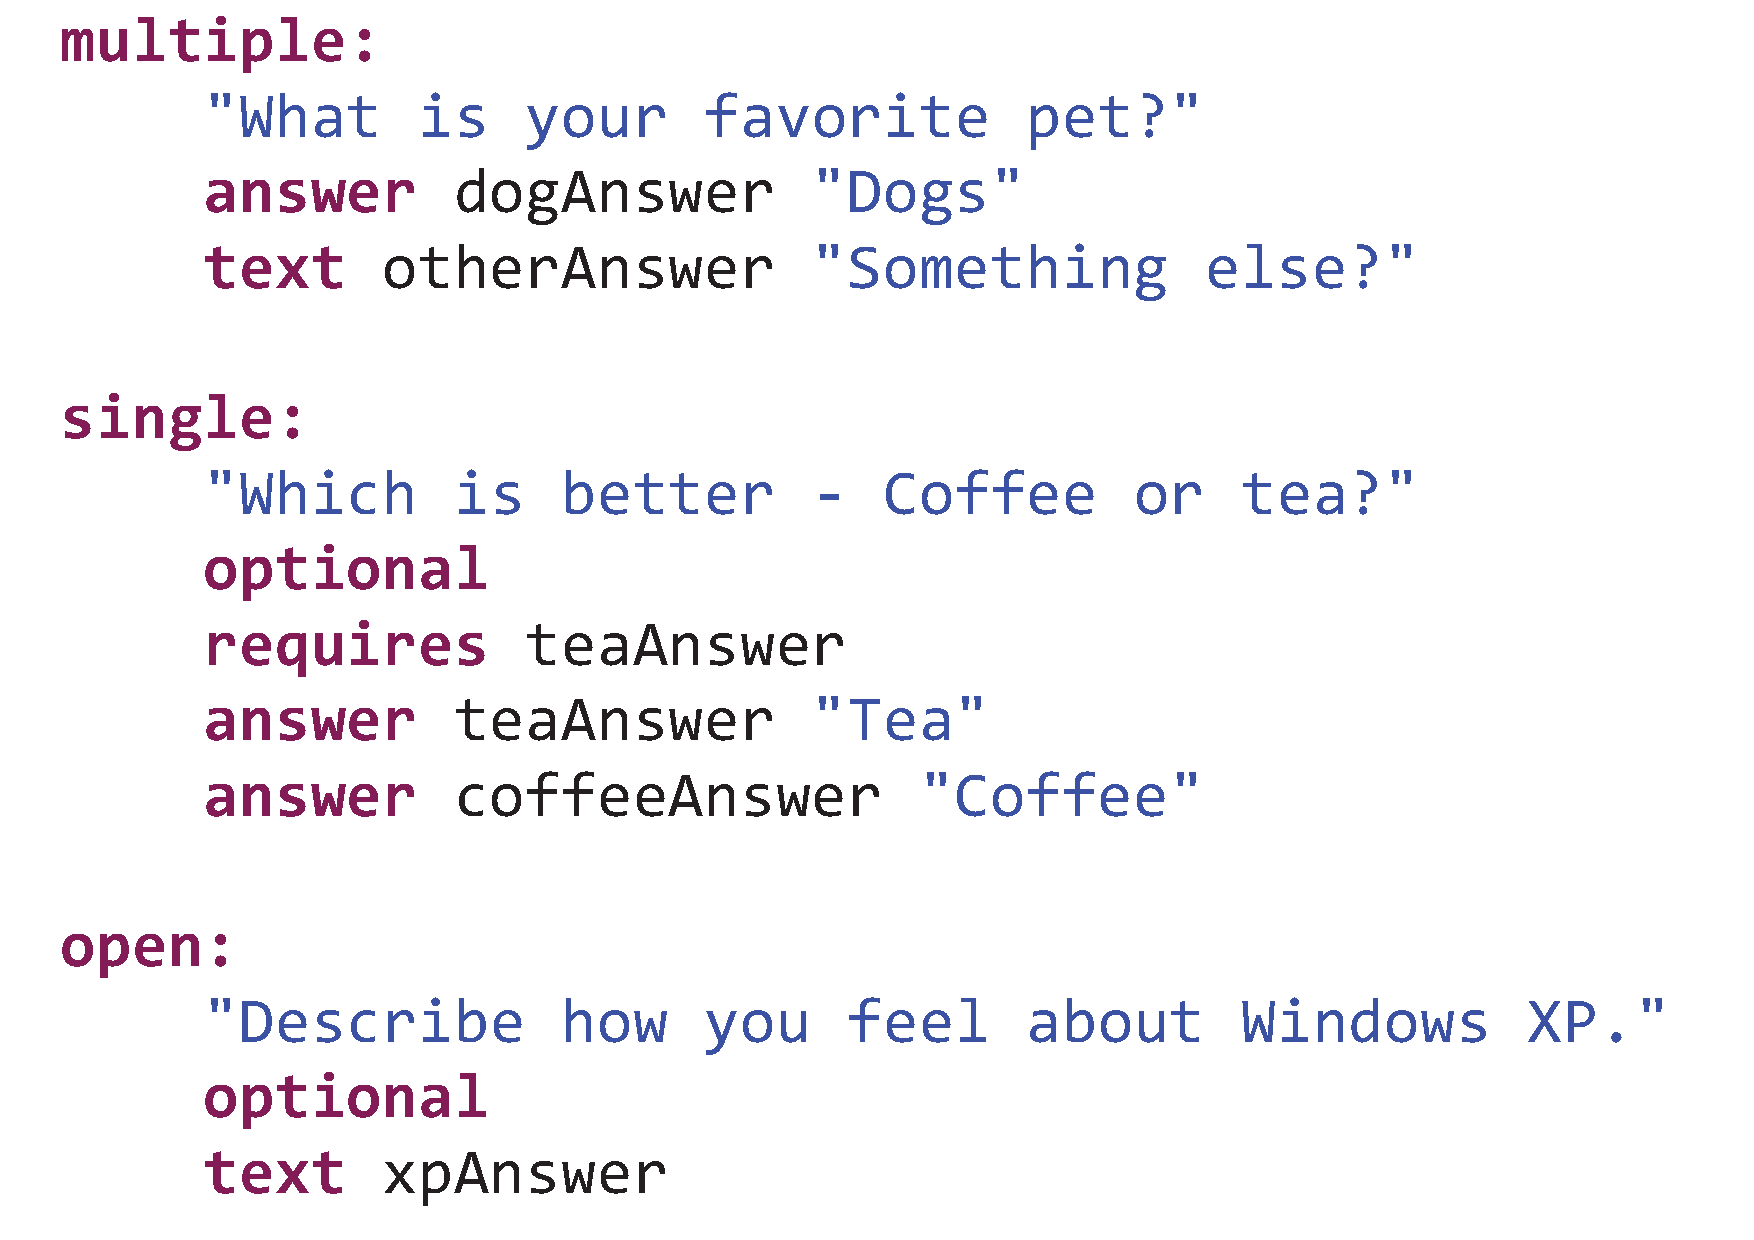
\includegraphics[height=5cm]{concretefail}
\caption{Faulty concrete syntax example.}
\label{fig:concretefail}
\end{figure}
\subsubsection{Unit Tests}
Unit tests are included in the auto-generated test project belonging to the DSL. These are written in Xtend and uses the jUnit framework. Two *.survey test instances are included in the test project and used in the tests. Given a *.survey file, the tests parse the files and check that the entities are correctly structured and contain the expected information. 
\subsection{Code Generation}
The testing of the code generation is purely manual. The general procedure was to generate the files and see if they could be used as intended. A brief description of the procedures is provided below.
\subsubsection{Android Application}
The generated code for the Android application has been manually tested by exporting the generated activity file into a new empty Android code project. The project is built and run on an emulator and on a Samsung Galaxy S3 Mini. We simulated a surveyee by answering the questions and checking the validity of each question- and answer description before submitting the data. Unfortunately, we found a significant flaw in the Java code - a question can only require a single previous answer. Because this error was discovered late in the process and the solution would require a relatively large restructure of the code, we had to leave it for further work. 
\subsubsection{Web application}
The generated code the Web application is tested using an HTML Verifier. Once the HTML file is produced, the file is checked by the HTML Verifier. The verifier tries to open the target file and tests that:
\begin{enumerate}
\item the file exists
\item the correct \texttt{<title>} title is given
\item the correct number of questions can be found
\item the correct \texttt{<form>} controls exist
\item the e-mail address of the \texttt{<form>}, towards which the information is send is correct
\end{enumerate}
Further manual testing was done by opening the generated file in a browser and checking that the layout and validation-checking behaves as intended.

\section{Further Work}
In order to further improve the functionality of the system we could have expanded the meta-model to include answer expressions. For instance, this would make a question's required previous answers more flexible by allowing them to be written as a boolean expression. Furthermore, we do not believe the testing is sufficient, namely, the testing of the code generation falls short. We would have liked to test the generated files automatically. The generated Android application should also support questions requiring more than one previous answer. Finally, we should have permitted comments in our language, as suggested by \cite{karsai}. Ultimately, the reasons for not adding the improvements are either due to reduced workforce, discovering them late in the project, or time constraints.

\section{Conclusion}
We have successfully modeled and implemented a DSL used to write surveys.
A domain analysis of popular online survey platforms was performed as a basis for the design of our DSL.
The DSL uses a simplistic syntax making it possible for domain experts without programming knowledge able to construct survey applications. 
These applications target two different platforms, namely the Android mobile platform and a Web platform. The DSL comes with an editor integrated within the Eclipse IDE. The editor provides syntax highlighting, constraint- and error checking.

The requirements for the DSL listed in section \ref{sec:requirements_and_design} are fully satisfied. However not all of the requirements are reflected in the implementation for the platforms. 

\begin{thebibliography}{4}

\bibitem{mernik} Mernik, M., Heering, J., Sloane, A. M.: When and how to develop domain-specific languages. ACM Comput. Surv., 37(4):316–344, 2005.

\bibitem{fowler}  Fowler, M., Parsons, R.: Domain-Specific Languages. Addison-Wesley, 2011.

\bibitem{karsai} Karsai, G., Krahn, H., Pinkernell, C.,, Rumpe, B., Schindler, M., Völkel, S.: Design guidelines for domain specific languages. 
9th OOPSLA Workshop on Domain-Specific Modeling (2009), \url{http://www.dsmforum.org/events/dsm09/Papers/Karsai.pdf}

\bibitem{surveymonkey}SurveyMonkey, \url{http://www.surveymonkey.com/s/Public-School-Survey-Template}

\bibitem{obsurvey}Obsurvey, \url{http://www.obsurvey.com/language-proficiency-template/}

\bibitem{xtext}Xtext, \url{http://www.eclipse.org/Xtext/}

\bibitem{xtend}Xtend, \url{http://www.eclipse.org/xtend/}

\end{thebibliography}

\end{document}
